\section{Zielsetzung}
Es soll mittels Sagnac Interferometer der Brechungsindex von Luft und Quarzglas bestimmt werden.,

\section{Theorie}
\subsection{Brechungsindex}
Der Brechungsindex $n$ eines Mediums bestimmt sich aus dem Verhältnis der Lichtgeschwindigkeit zur Phasengeschwindigkeit der durch das Medium
propagierende Welle.

\begin{equation}
n = \frac{c}{v_{ph}}
\end{equation}

wobei die Phasengeschwindigkeit einer Welle sich aus Kreisfrequenz $\omega$ und Wellenzahl $k$ bestimmt.

\begin{equation}
v_{ph} = \frac{\omega}{k}
\end{equation}

Im allgemeinen ist eine Welle ein Objekt, welches sich in Ort und Zeit periodisch ändert. Mathematisch wird dieses Verhalten durch eine komplexe
e-Funktion beschrieben

\begin{equation}
f(x, t) = A\exp{i(kx - wt)} = A \exp{ikx} \exp{-iwt}
\end{equation}

wobei der erste Exponentialterm die Phasenänderung beschreibt und der zweite Exponentialterm, auch Phasor genannt, die zeitliche Änderung der Welle berücksichtigt.
Wird zusätzlich die Kreisfrequenz durch die Wellenlänge im Vakuum ausgedrückt, können wir die Phasenänderung pro Länge durch die Brechzahl ausdrücken.

\begin{equation}
f(x, t) = A \exp{-i\omega t} \exp{2 \pi i \frac{n}{\lambda_{vac}} x}
\end{equation}

Die Phasendifferenz zweier Wellen, welche durch das Vakuum mit $n=1$ und einem Medium mit der Brechzahl $n$ und der Länge L propagiert, errechnet sich zu

\begin{equation}
\delta \phi = \frac{2 \pi}{\lambda_{vac}} \delta n L = \frac{2 \pi}{\lambda_{vac}} (n - 1)L.
\end{equation}

Die Anzahl der Intensitätsmaxima N ergibt sich aus der Phasendifferenz

\begin{equation}
N=\frac{\delta \phi}{2 \pi} = \frac{n-1}{\lambda_{vac}} L.
\end{equation}

Um die Auswirkung von Druck oder Temperaturänderungen auf die Brechzahl berücksichtigen zu können, wird das Lorenz-Lorentz Gesetz

\begin{equation}
	n = \sqrt{1 + \frac{3Ap}{RT}}
\end{equation}

genutzt.

\subsection{Strahlengang durch ein Glasplättchen}

% Abbildung noch nicht aktuell
%\begin{figure}[h]
%\centering
%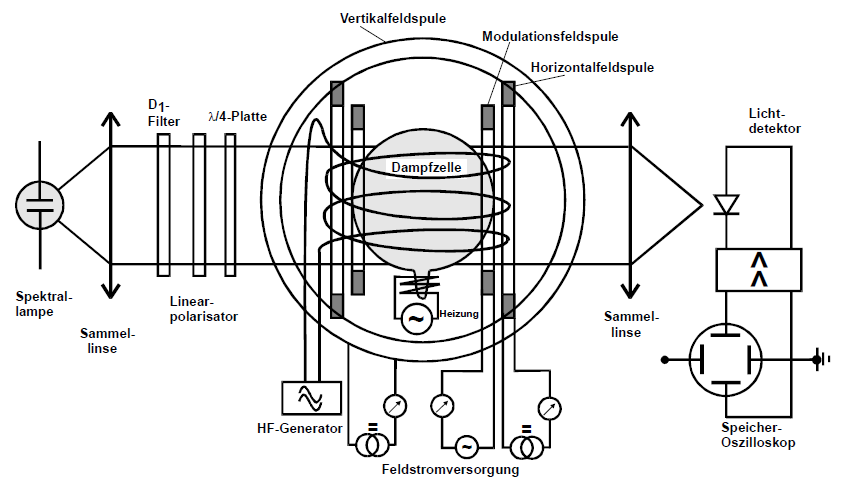
\includegraphics[scale=0.8]{./optischesPumpen/img/aufbau.png}
%\caption{Schematischer Aufbau der Versuchsapparatur [1]}
%\label{aufbau}
%\end{figure}

Die Messung der Brechzahl von Quarzglas basiert auf dem Gangunterschied, welcher das Licht erfährt, wenn es durch das Medium propagiert.
Der Gangunterschied hängt im wesentlichen von dem Brechzahlsprung an der Grenzfläche des Mediums und dem Auslenkungswinkel ab.

\begin{equation}
\phi(\Phi) = \frac{2 \pi}{\lambda_{vac}} \left( \frac{n_2 - n_1 \cos(\Phi - \Phi')}{\cos(\Phi')} - \frac{n_2 - n_1}{n_1}\right)
\end{equation}

\subsection{Kontrast}
Der Kontrast eines Interferometers ist ein Maß für die Interferenzfähikeit des Lichtest. Der Kontrast ist durch

\begin{equation}
K = \frac{|I_{max} - I_{min}|}{|I_{max} + I_{min}|}
\end{equation}

Der Kontrast hängt maßgeblich vom Polarisationswinkel des Polarisators vor dem Interferometer ab.
\begin{equation}
K = C|\cos(\phi + \delta) * \sin(\phi + \delta)|
\end{equation}
